\documentclass[11pt]{article}

\usepackage{amsmath,amssymb,latexsym}
\usepackage{amsmath,amsthm,amsfonts,amssymb,amscd,enumerate,upgreek,dsfont}
\usepackage{graphicx}
\usepackage{wrapfig}
\usepackage{subfig}
\usepackage[margin=1in]{geometry}



\newtheorem{thm}{Theorem}
\newtheorem{prop}[thm]{Proposition}
\newtheorem{asp}[thm]{Assumption}
\newtheorem{defn}[thm]{Definition}
\newtheorem{lemma}[thm]{Lemma}
\newtheorem{obs}[thm]{Observation}
\newtheorem{cor}[thm]{Corollary}
\newtheorem{fact}[thm]{Fact}
\newtheorem{remark}[thm]{Remark}
\newtheorem{eg}[thm]{Example}

\newenvironment{pack_enum}{
	\begin{enumerate}
		\setlength{\itemsep}{0pt}
		\setlength{\parskip}{0pt}
		\setlength{\parsep}{0pt}}{\end{enumerate}
}

\newenvironment{pack_item}{
	\begin{itemize}
		\setlength{\itemsep}{0pt}
		\setlength{\parskip}{0pt}
		\setlength{\parsep}{0pt}}{\end{itemize}
}



\newenvironment{enum_label}{
	\begin{enumerate}[label=\textnormal{(\arabic*)}]
	}{\end{enumerate}
}



%%%%%%%%%%%%%%%%% THEOREM and PROOF
%\numberwithin{equation}{section}

\newcommand{\BeginPf}{\noindent {\em Proof: }} % Start Proof
\newcommand{\EndPf}{\hfill $\square$ }     % End of proof symbol


%%%%%%%%%%%%%%%%%
\newcommand{\bA}{\mathbb{A}}
\newcommand{\bB}{\mathbb{B}}
\newcommand{\bC}{\mathbb{C}}
\newcommand{\bD}{\mathbb{D}}
\newcommand{\bE}{\mathbb{E}}
\newcommand{\bF}{\mathbb{F}}
\newcommand{\bG}{\mathbb{G}}
\newcommand{\bH}{\mathbb{H}}
\newcommand{\bI}{\mathbb{I}}
\newcommand{\bJ}{\mathbb{J}}
\newcommand{\bL}{\mathbb{L}}
\newcommand{\bK}{\mathbb{K}}
\newcommand{\bM}{\mathbb{M}}
\newcommand{\bN}{\mathbb{N}}
\newcommand{\bO}{\mathbb{O}}
\newcommand{\bP}{\mathbb{P}}
\newcommand{\bQ}{\mathbb{Q}}
\newcommand{\bR}{\mathbb{R}}
\newcommand{\bS}{\mathbb{S}}
\newcommand{\bT}{\mathbb{T}}
\newcommand{\bU}{\mathbb{U}}
\newcommand{\bV}{\mathbb{V}}
\newcommand{\bW}{\mathbb{W}}
\newcommand{\bX}{\mathbb{X}}
\newcommand{\bY}{\mathbb{Y}}
\newcommand{\bZ}{\mathbb{Z}}

\newcommand{\Prob}{\text{Prob}}
\newcommand{\dist}{\text{dist}}
\newcommand{\wpo}{\text{w.p.1}}

\newcommand{\sA}{\mathscr{A}}
\newcommand{\sB}{\mathscr{B}}
\newcommand{\sC}{\mathscr{C}}
\newcommand{\sD}{\mathscr{D}}
\newcommand{\sE}{\mathscr{E}}
\newcommand{\sF}{\mathscr{F}}
\newcommand{\sG}{\mathscr{G}}
\newcommand{\sH}{\mathscr{H}}
\newcommand{\sI}{\mathscr{I}}
\newcommand{\sJ}{\mathscr{J}}
\newcommand{\sL}{\mathscr{L}}
\newcommand{\sK}{\mathscr{K}}
\newcommand{\sM}{\mathscr{M}}
\newcommand{\sN}{\mathscr{N}}
\newcommand{\sO}{\mathscr{O}}
\newcommand{\sP}{\mathscr{P}}
\newcommand{\sQ}{\mathscr{Q}}
\newcommand{\sR}{\mathscr{R}}
\newcommand{\sS}{\mathscr{S}}
\newcommand{\sT}{\mathscr{T}}
\newcommand{\sU}{\mathscr{U}}
\newcommand{\sV}{\mathscr{V}}
\newcommand{\sW}{\mathscr{W}}
\newcommand{\sX}{\mathscr{X}}
\newcommand{\sY}{\mathscr{Y}}
\newcommand{\sZ}{\mathscr{Z}}

\newcommand{\cA}{\mathcal{A}}
\newcommand{\cB}{\mathcal{B}}
\newcommand{\cC}{\mathcal{C}}
\newcommand{\cD}{\mathcal{D}}
\newcommand{\cE}{\mathcal{E}}
\newcommand{\cF}{\mathcal{F}}
\newcommand{\cG}{\mathcal{G}}
\newcommand{\cH}{\mathcal{H}}
\newcommand{\cI}{\mathcal{I}}
\newcommand{\cJ}{\mathcal{J}}
\newcommand{\cL}{\mathcal{L}}
\newcommand{\cK}{\mathcal{K}}
\newcommand{\cM}{\mathcal{M}}
\newcommand{\cN}{\mathcal{N}}
\newcommand{\cO}{\mathcal{O}}
\newcommand{\cP}{\mathcal{P}}
\newcommand{\cQ}{\mathcal{Q}}
\newcommand{\cR}{\mathcal{R}}
\newcommand{\cS}{\mathcal{S}}
\newcommand{\cT}{\mathcal{T}}
\newcommand{\cU}{\mathcal{U}}
\newcommand{\cV}{\mathcal{V}}
\newcommand{\cW}{\mathcal{W}}
\newcommand{\cX}{\mathcal{X}}
\newcommand{\cY}{\mathcal{Y}}
\newcommand{\cZ}{\mathcal{Z}}


\newcommand{\fA}{\mathfrak{A}}
\newcommand{\fB}{\mathfrak{B}}
\newcommand{\fC}{\mathfrak{C}}
\newcommand{\fD}{\mathfrak{D}}
\newcommand{\fE}{\mathfrak{E}}
\newcommand{\fF}{\mathfrak{F}}
\newcommand{\fG}{\mathfrak{G}}
\newcommand{\fH}{\mathfrak{H}}
\newcommand{\fI}{\mathfrak{I}}
\newcommand{\fJ}{\mathfrak{J}}
\newcommand{\fL}{\mathfrak{L}}
\newcommand{\fK}{\mathfrak{K}}
\newcommand{\fM}{\mathfrak{M}}
\newcommand{\fN}{\mathfrak{N}}
\newcommand{\fO}{\mathfrak{O}}
\newcommand{\fP}{\mathfrak{P}}
\newcommand{\fQ}{\mathfrak{Q}}
\newcommand{\fR}{\mathfrak{R}}
\newcommand{\fS}{\mathfrak{S}}
\newcommand{\fT}{\mathfrak{T}}
\newcommand{\fU}{\mathfrak{U}}
\newcommand{\fV}{\mathfrak{V}}
\newcommand{\fW}{\mathfrak{W}}
\newcommand{\fX}{\mathfrak{X}}
\newcommand{\fY}{\mathfrak{Y}}
\newcommand{\fZ}{\mathfrak{Z}}



\newcommand{\fa}{\mathfrak{a}}
\newcommand{\fb}{\mathfrak{b}}
\newcommand{\fc}{\mathfrak{c}}
\newcommand{\fd}{\mathfrak{d}}
\newcommand{\fe}{\mathfrak{e}}
\newcommand{\ff}{\mathfrak{f}}
\newcommand{\fg}{\mathfrak{g}}
\newcommand{\fh}{\mathfrak{h}}
%\newcommand{\fi}{\mathfrak{i}}  % \fi is already a TeX primitive
\newcommand{\fj}{\mathfrak{j}}
\newcommand{\fk}{\mathfrak{k}}
\newcommand{\fl}{\mathfrak{l}}
\newcommand{\fm}{\mathfrak{m}}
\newcommand{\fn}{\mathfrak{n}}
\newcommand{\fo}{\mathfrak{o}}
\newcommand{\fp}{\mathfrak{p}}
\newcommand{\fq}{\mathfrak{q}}
\newcommand{\fr}{\mathfrak{r}}
\newcommand{\fs}{\mathfrak{s}}
\newcommand{\ft}{\mathfrak{t}}
\newcommand{\fu}{\mathfrak{u}}
\newcommand{\fv}{\mathfrak{v}}
\newcommand{\fw}{\mathfrak{w}}
\newcommand{\fx}{\mathfrak{x}}
\newcommand{\fy}{\mathfrak{y}}
\newcommand{\fz}{\mathfrak{z}}

\newcommand{\one}{\mathds{1}}
\newcommand{\dA}{\mathds{A}}
\newcommand{\dB}{\mathds{B}}
\newcommand{\dC}{\mathds{C}}
\newcommand{\dD}{\mathds{D}}
\newcommand{\dE}{\mathds{E}}
\newcommand{\dF}{\mathds{F}}
\newcommand{\dG}{\mathds{G}}
\newcommand{\dH}{\mathds{H}}
\newcommand{\dI}{\mathds{I}}
\newcommand{\dJ}{\mathds{J}}
\newcommand{\dL}{\mathds{L}}
\newcommand{\dK}{\mathds{K}}
\newcommand{\dM}{\mathds{M}}
\newcommand{\dN}{\mathds{N}}
\newcommand{\dO}{\mathds{O}}
\newcommand{\dP}{\mathds{P}}
\newcommand{\dQ}{\mathds{Q}}
\newcommand{\dR}{\mathds{R}}
\newcommand{\dS}{\mathds{S}}
\newcommand{\dT}{\mathds{T}}
\newcommand{\dU}{\mathds{U}}
\newcommand{\dV}{\mathds{V}}
\newcommand{\dW}{\mathds{W}}
\newcommand{\dX}{\mathds{X}}
\newcommand{\dY}{\mathds{Y}}
\newcommand{\dZ}{\mathds{Z}}

%%%%%%%%%%%%%%%%% FUNCTIONS
\newcommand{\step}[1]{\mathbb{1}\left\{#1\right\}}
\newcommand{\prob}[1]{\text{Pr}\left\{#1\right\}}
\newcommand{\sd}{\trianglerighteq}

\newcommand{\jl}[1]{\text{\color{red}{#1}}}

%%%%%%%%%%%%%%%%% Matrix

\newlength{\dhatheight}
\newcommand{\doublehat}[1]{%
    \settoheight{\dhatheight}{\ensuremath{\hat{#1}}}%
    \addtolength{\dhatheight}{-0.35ex}%
    \hat{\vphantom{\rule{1pt}{\dhatheight}}%
    \smash{\hat{#1}}}}

\begin{document}
	\begin{eg}
	We consider a day-ahead charging model for an electric vehicle (EV) fleet where the goal is to minimize the total expected cost of charging the fleet under uncertain electricity prices and demand. The optimization model is formulated as follows:
	\begin{equation}
		\min_x \left\{ cx + \mathbb{E}_p[Q(x, \xi)] : cx < B, \ x \geq 0 \right\},
	\end{equation}
	where the cost function $Q(x, \xi)$ is given by
	\begin{equation}
		Q(x, \xi) := \min_y \left\{ s(D(\xi) - x - y) + W(\xi)y : W(\xi)y + cx \leq B, \ y \geq 0 \right\}.
	\end{equation}
	Here, $x$ represents the amount of eletricity to buy now and $y$ is the amount to buy tomorrow,   \( D(\xi) \) signifies the demand for electricity, which is dependent on the random variable \( \xi \), encapsulating the uncertainty in demand. The term \( W(\xi) \) reflects the price of electricity that can vary with \( \xi \). The penalty for unsatisfied demand is represented by \( s \). The decision variables \( x \) and \( y \) denote the electricity purchased a day ahead and on the day of operation, respectively.
	\end{eg}	
	
\noindent\textbf{{Numerical Test}.}
In our study, we set the unit price of buying electricity today as $c=1$. We differentiate between two types of scenarios: regular days and worst-case days. On regular days, the distributions for charging demand ($D(\xi)$) and price ($W(\xi)$) are characterized as follows:
\[
D(\xi) \sim \mathcal{U}(5,15), \quad W(\xi) \sim \mathcal{U}(0.5,1.5),
\]
where $\mathcal{U}(a,b)$ denotes the uniform distribution between $a$ and $b$. In the worst-case scenario, the mean values of these random variables are threefold compared to regular days, specifically:
\[
D(\xi) \sim 2\cdot\mathcal{U}(5,15), \quad W(\xi) \sim 2\cdot\mathcal{U}(0.5,1.5).
\]
The probabilities of encountering regular and worst-case days are also differentiated, with $P(\text{regular}) = 0.7$ and $P(\text{worst}) = 0.3$. The total buget $B$ is set to 10 and the penalty $s = 2.5$.

%\begin{figure}[htbp]
%	\begin{center}
%		\subfloat[$N = 10$  \label{fig:RR-N30}]{
%			\includegraphics[width=0.33\textwidth]{performance_vs_reliability_alpha_10.jpg}
%		}
%		\subfloat[$N = 30$ \label{fig:RR-N120}]{
%			\includegraphics[width=0.33\textwidth]{performance_vs_reliability_alpha_30.jpg}
%		}
%		\subfloat[$N = 70$ \label{fig:RR-N480}]{
%			\includegraphics[width=0.33\textwidth]{performance_vs_reliability_alpha_70.jpg}
%		}
%		\caption{The optimal value of our model is \textbf{29.7}. We now compare the result for Out-of-sample performance (left axis, solid line, and shaded area) and the coverage probability (right axis, dashed line) as a function of the nominal confidence level $(1-\alpha)$ in APUB-SP. The star symbol indicates the point where the mean of the out-of-sample performance attains its minimum.  } \label{fig:RR-APUB} 
%	\end{center}
%\end{figure}


\begin{figure}[htbp]
	\begin{center}
		\subfloat[$N = 20$  \label{fig:RR-N30}]{
			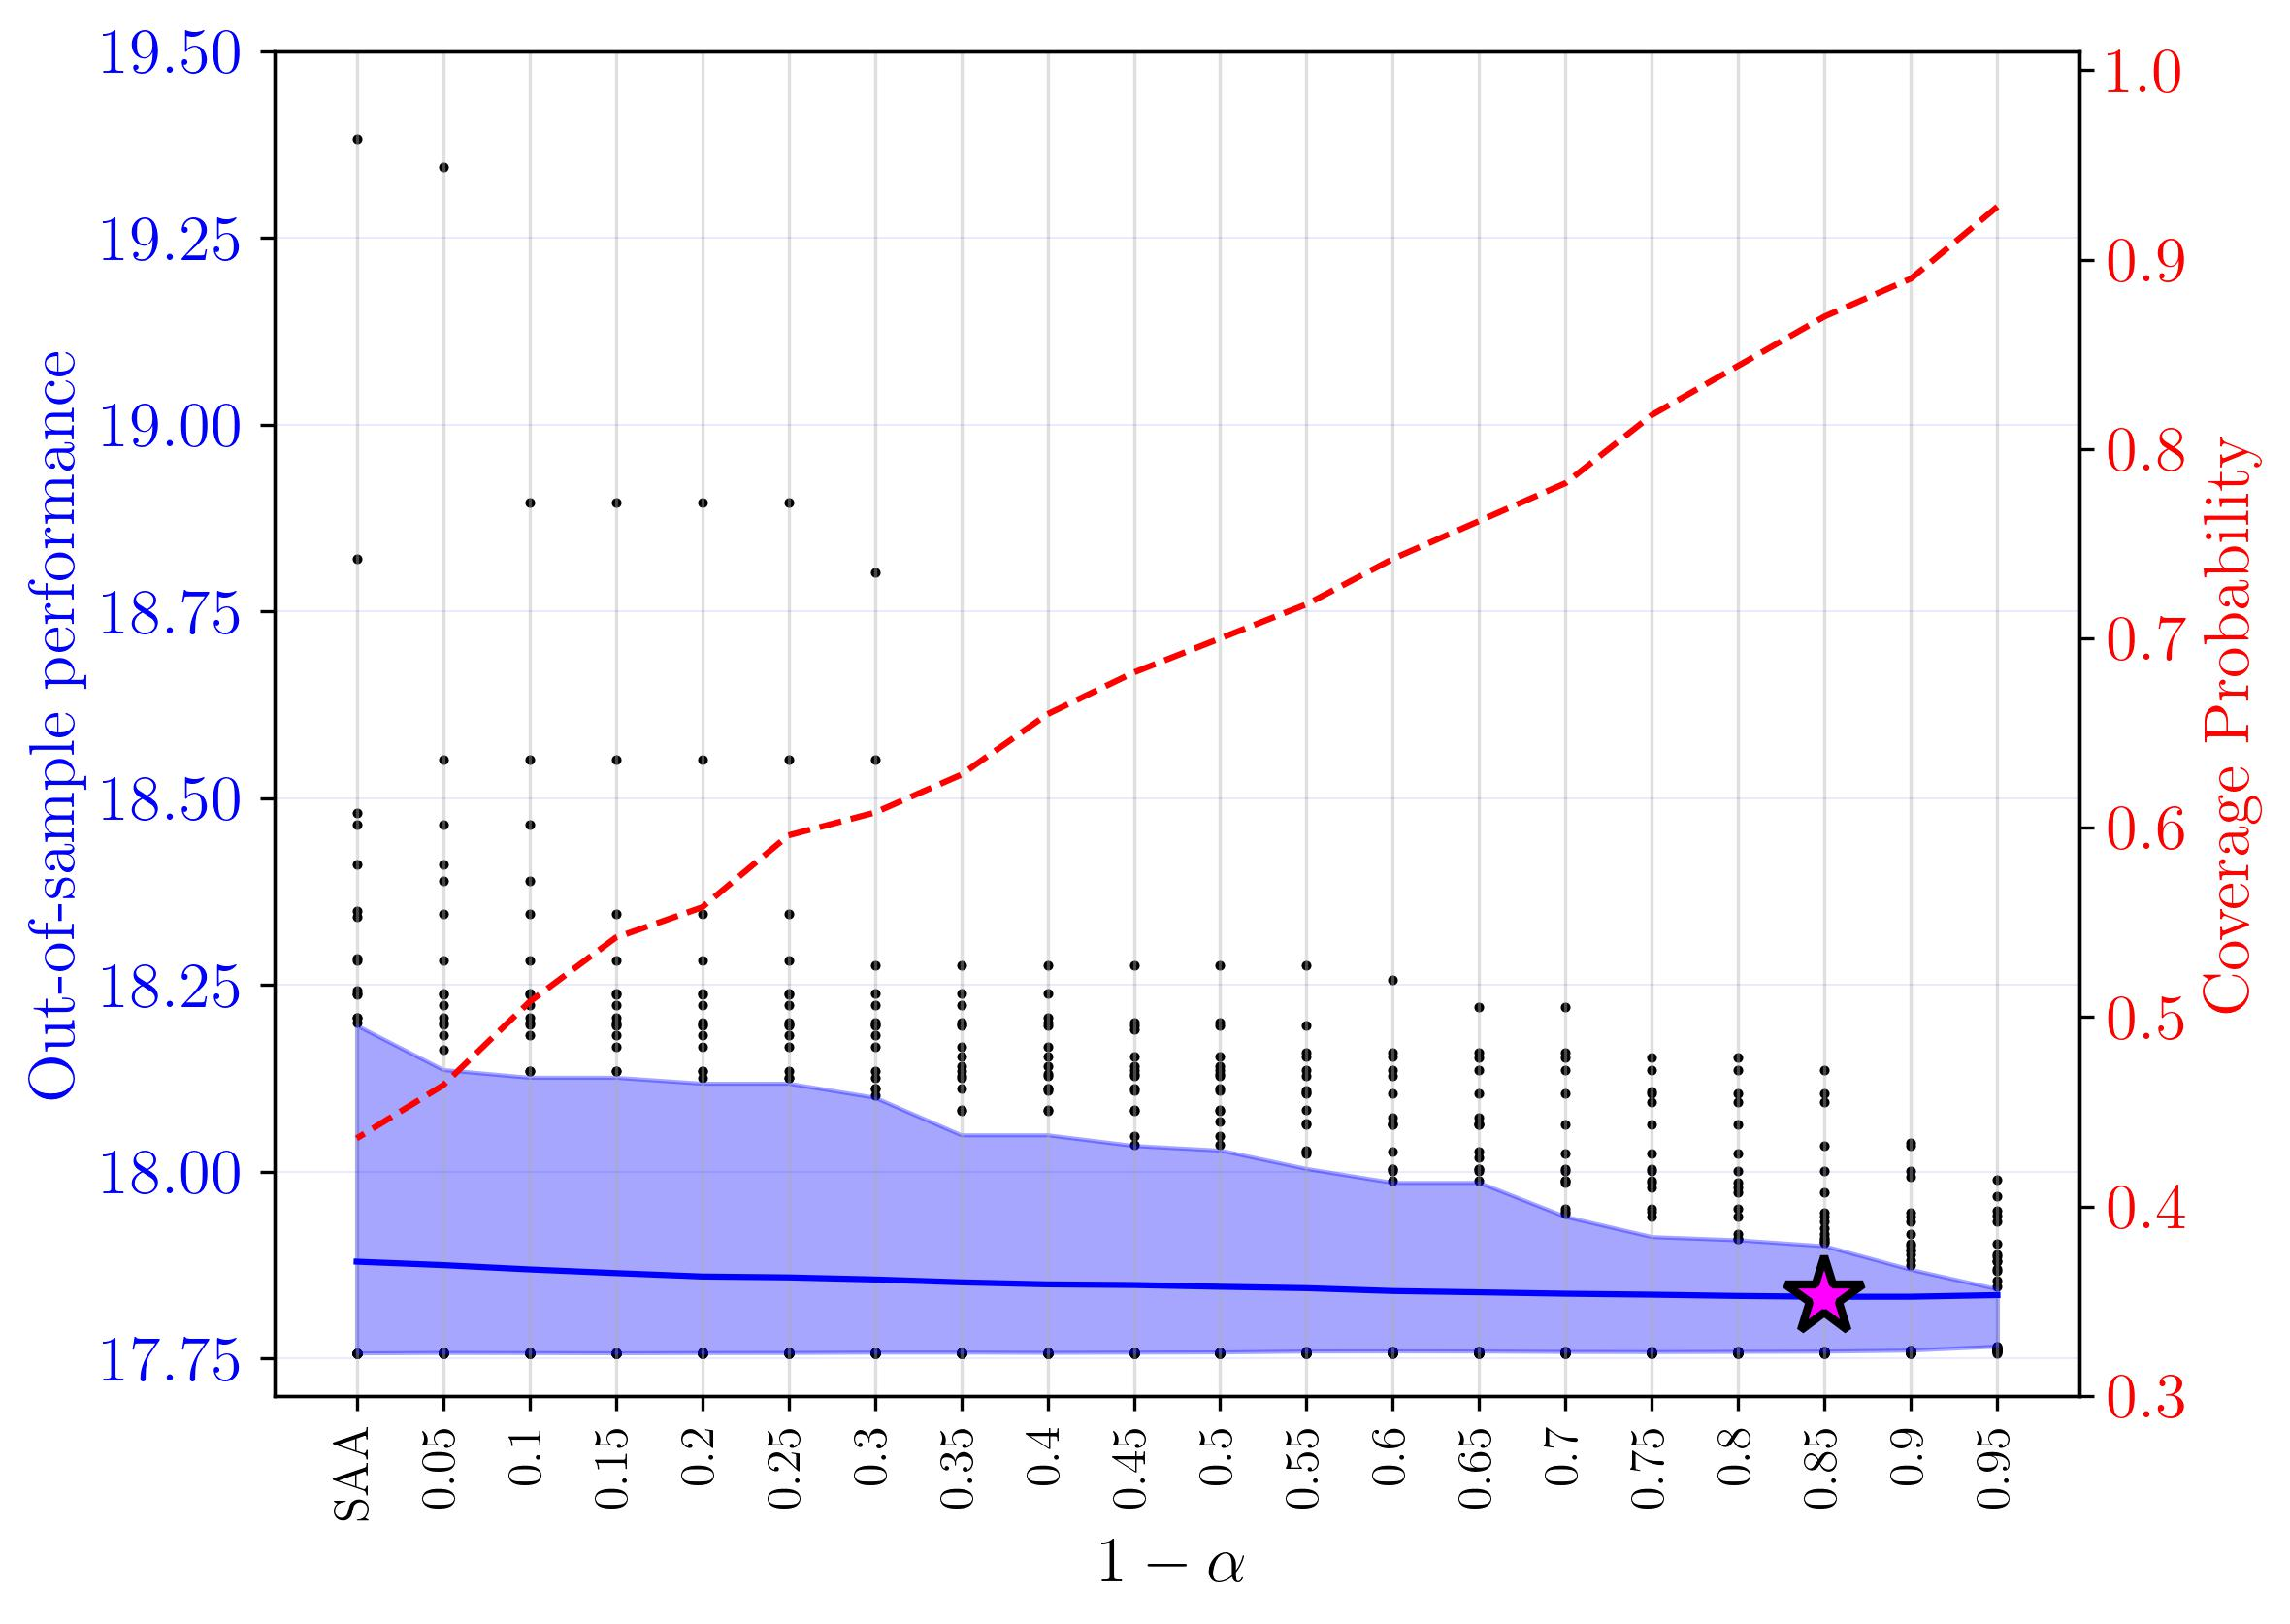
\includegraphics[width=0.33\textwidth]{performance_vs_reliability_alpha_20.jpg}
		}
		\subfloat[$N = 80$ \label{fig:RR-N480}]{
			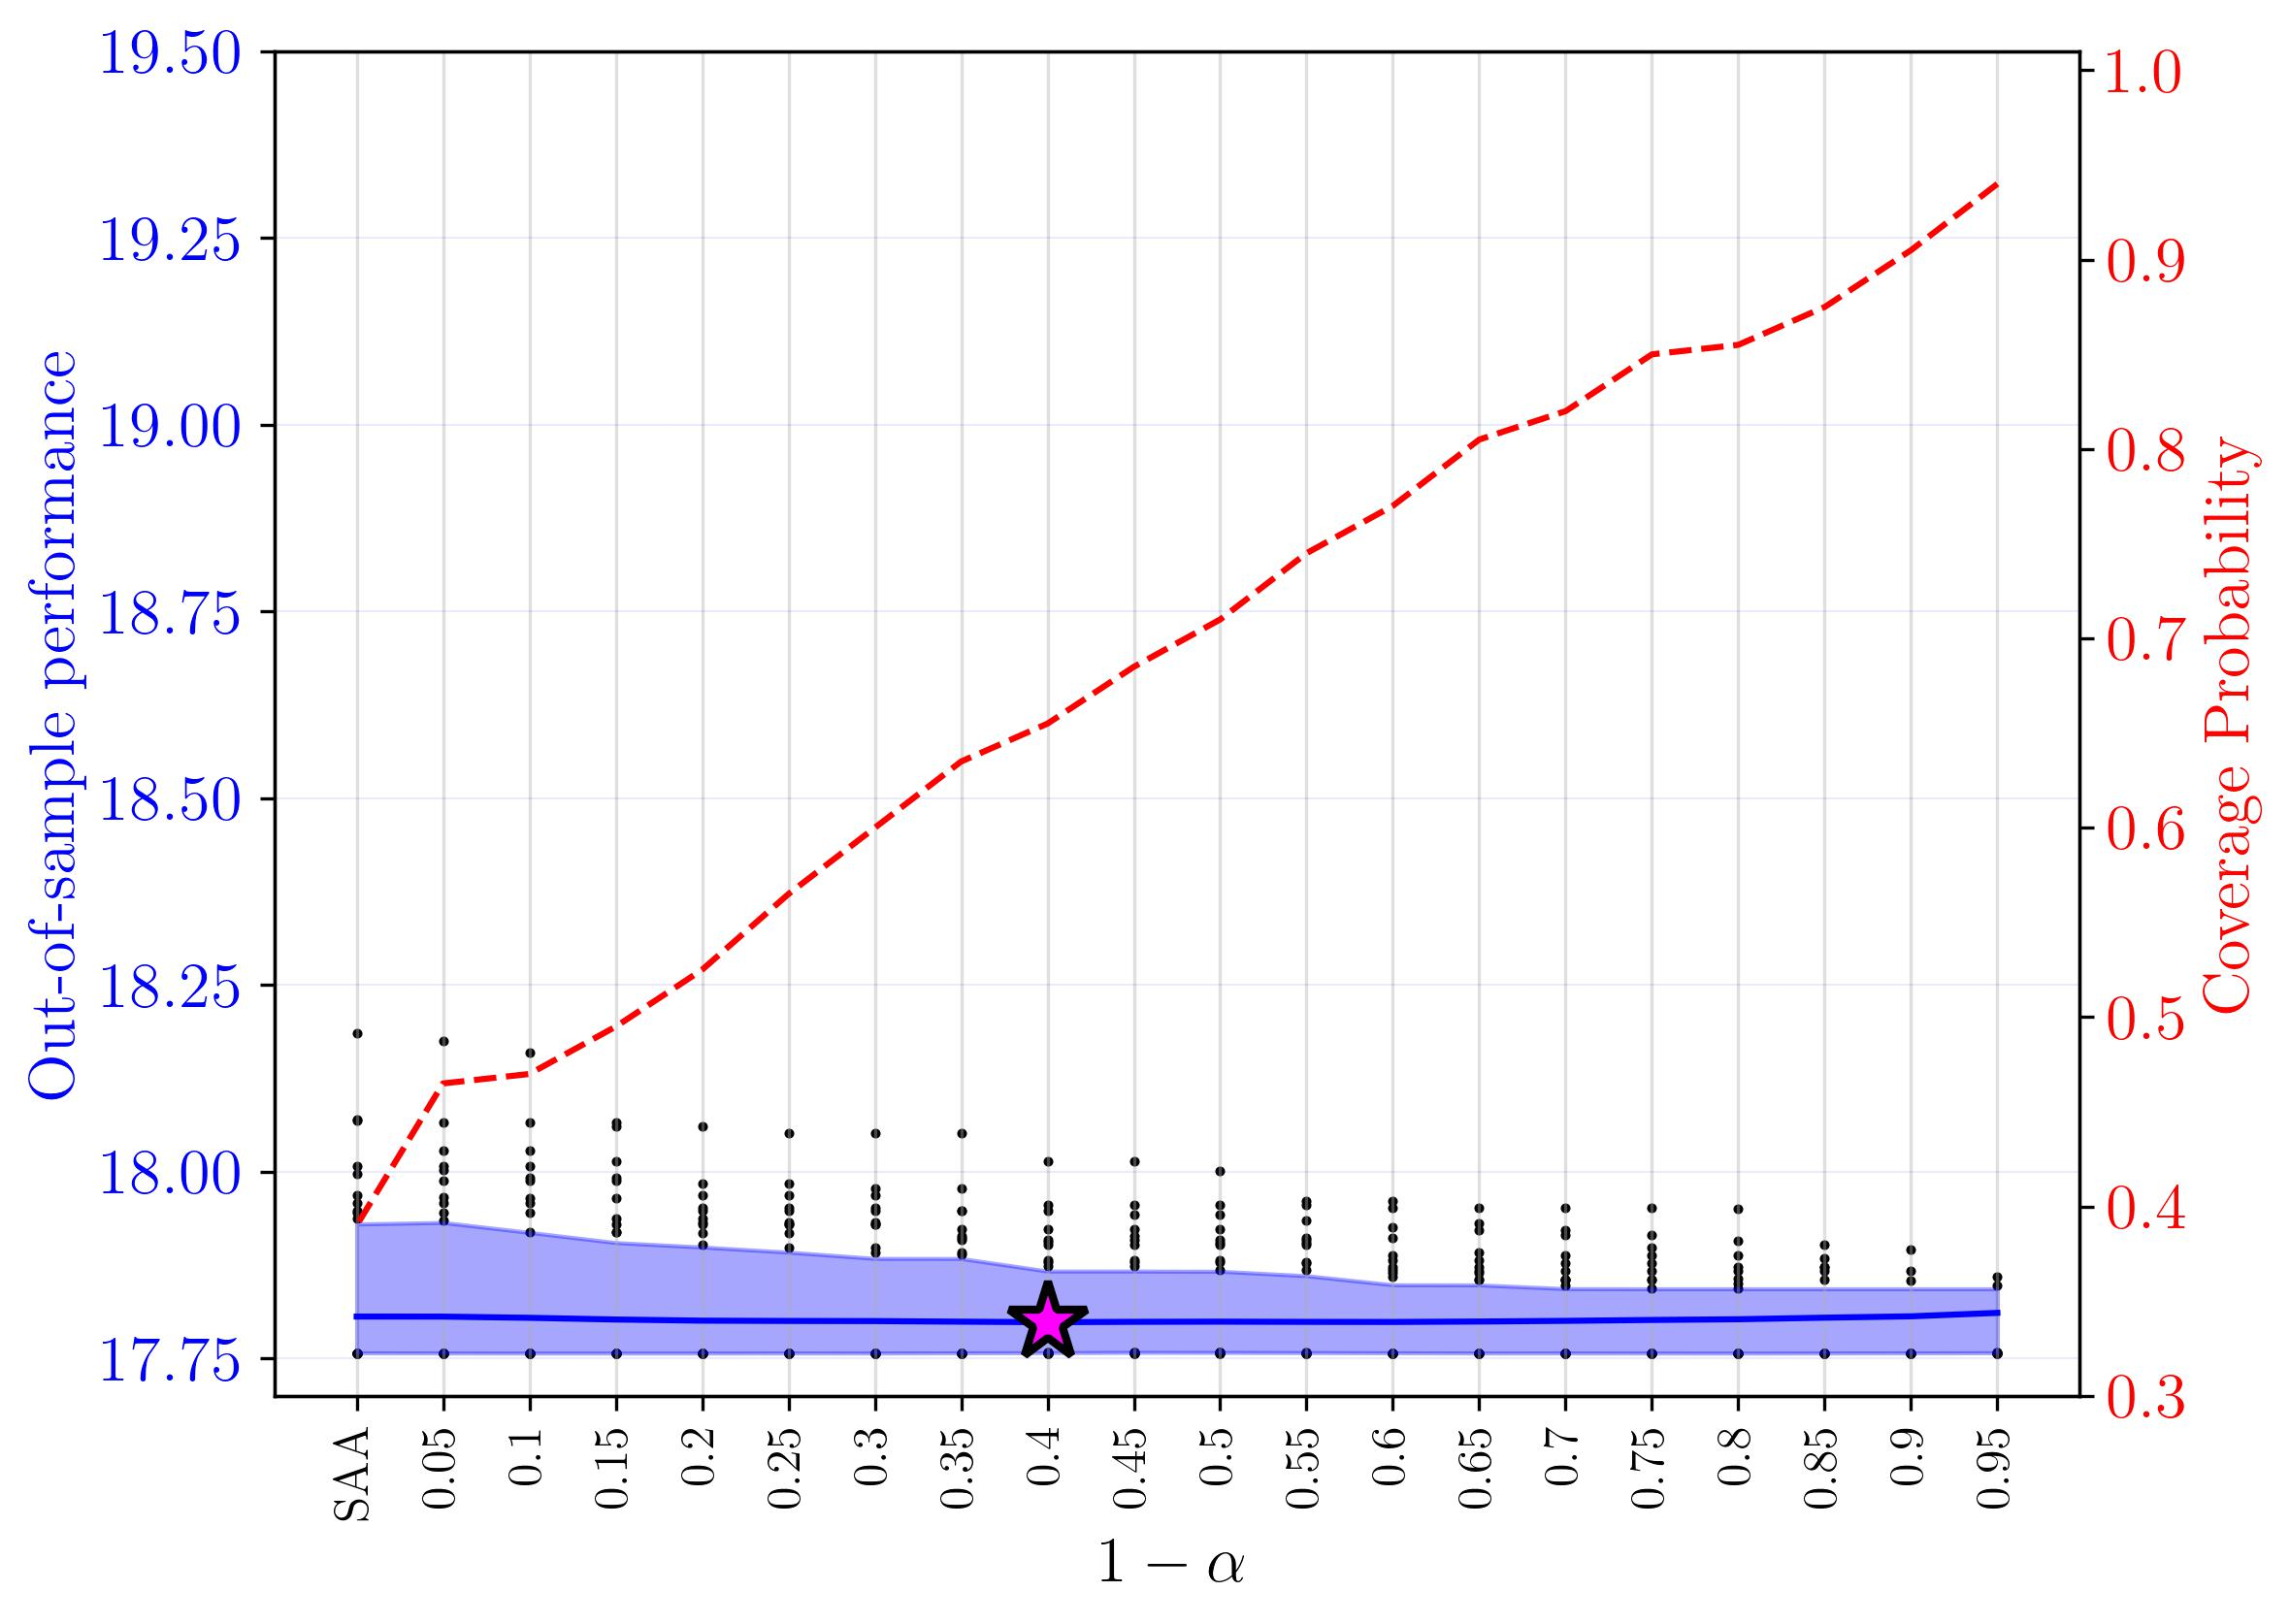
\includegraphics[width=0.33\textwidth]{performance_vs_reliability_alpha_80.jpg}
		}
		\subfloat[$N = 640$ \label{fig:RR-N120}]{
		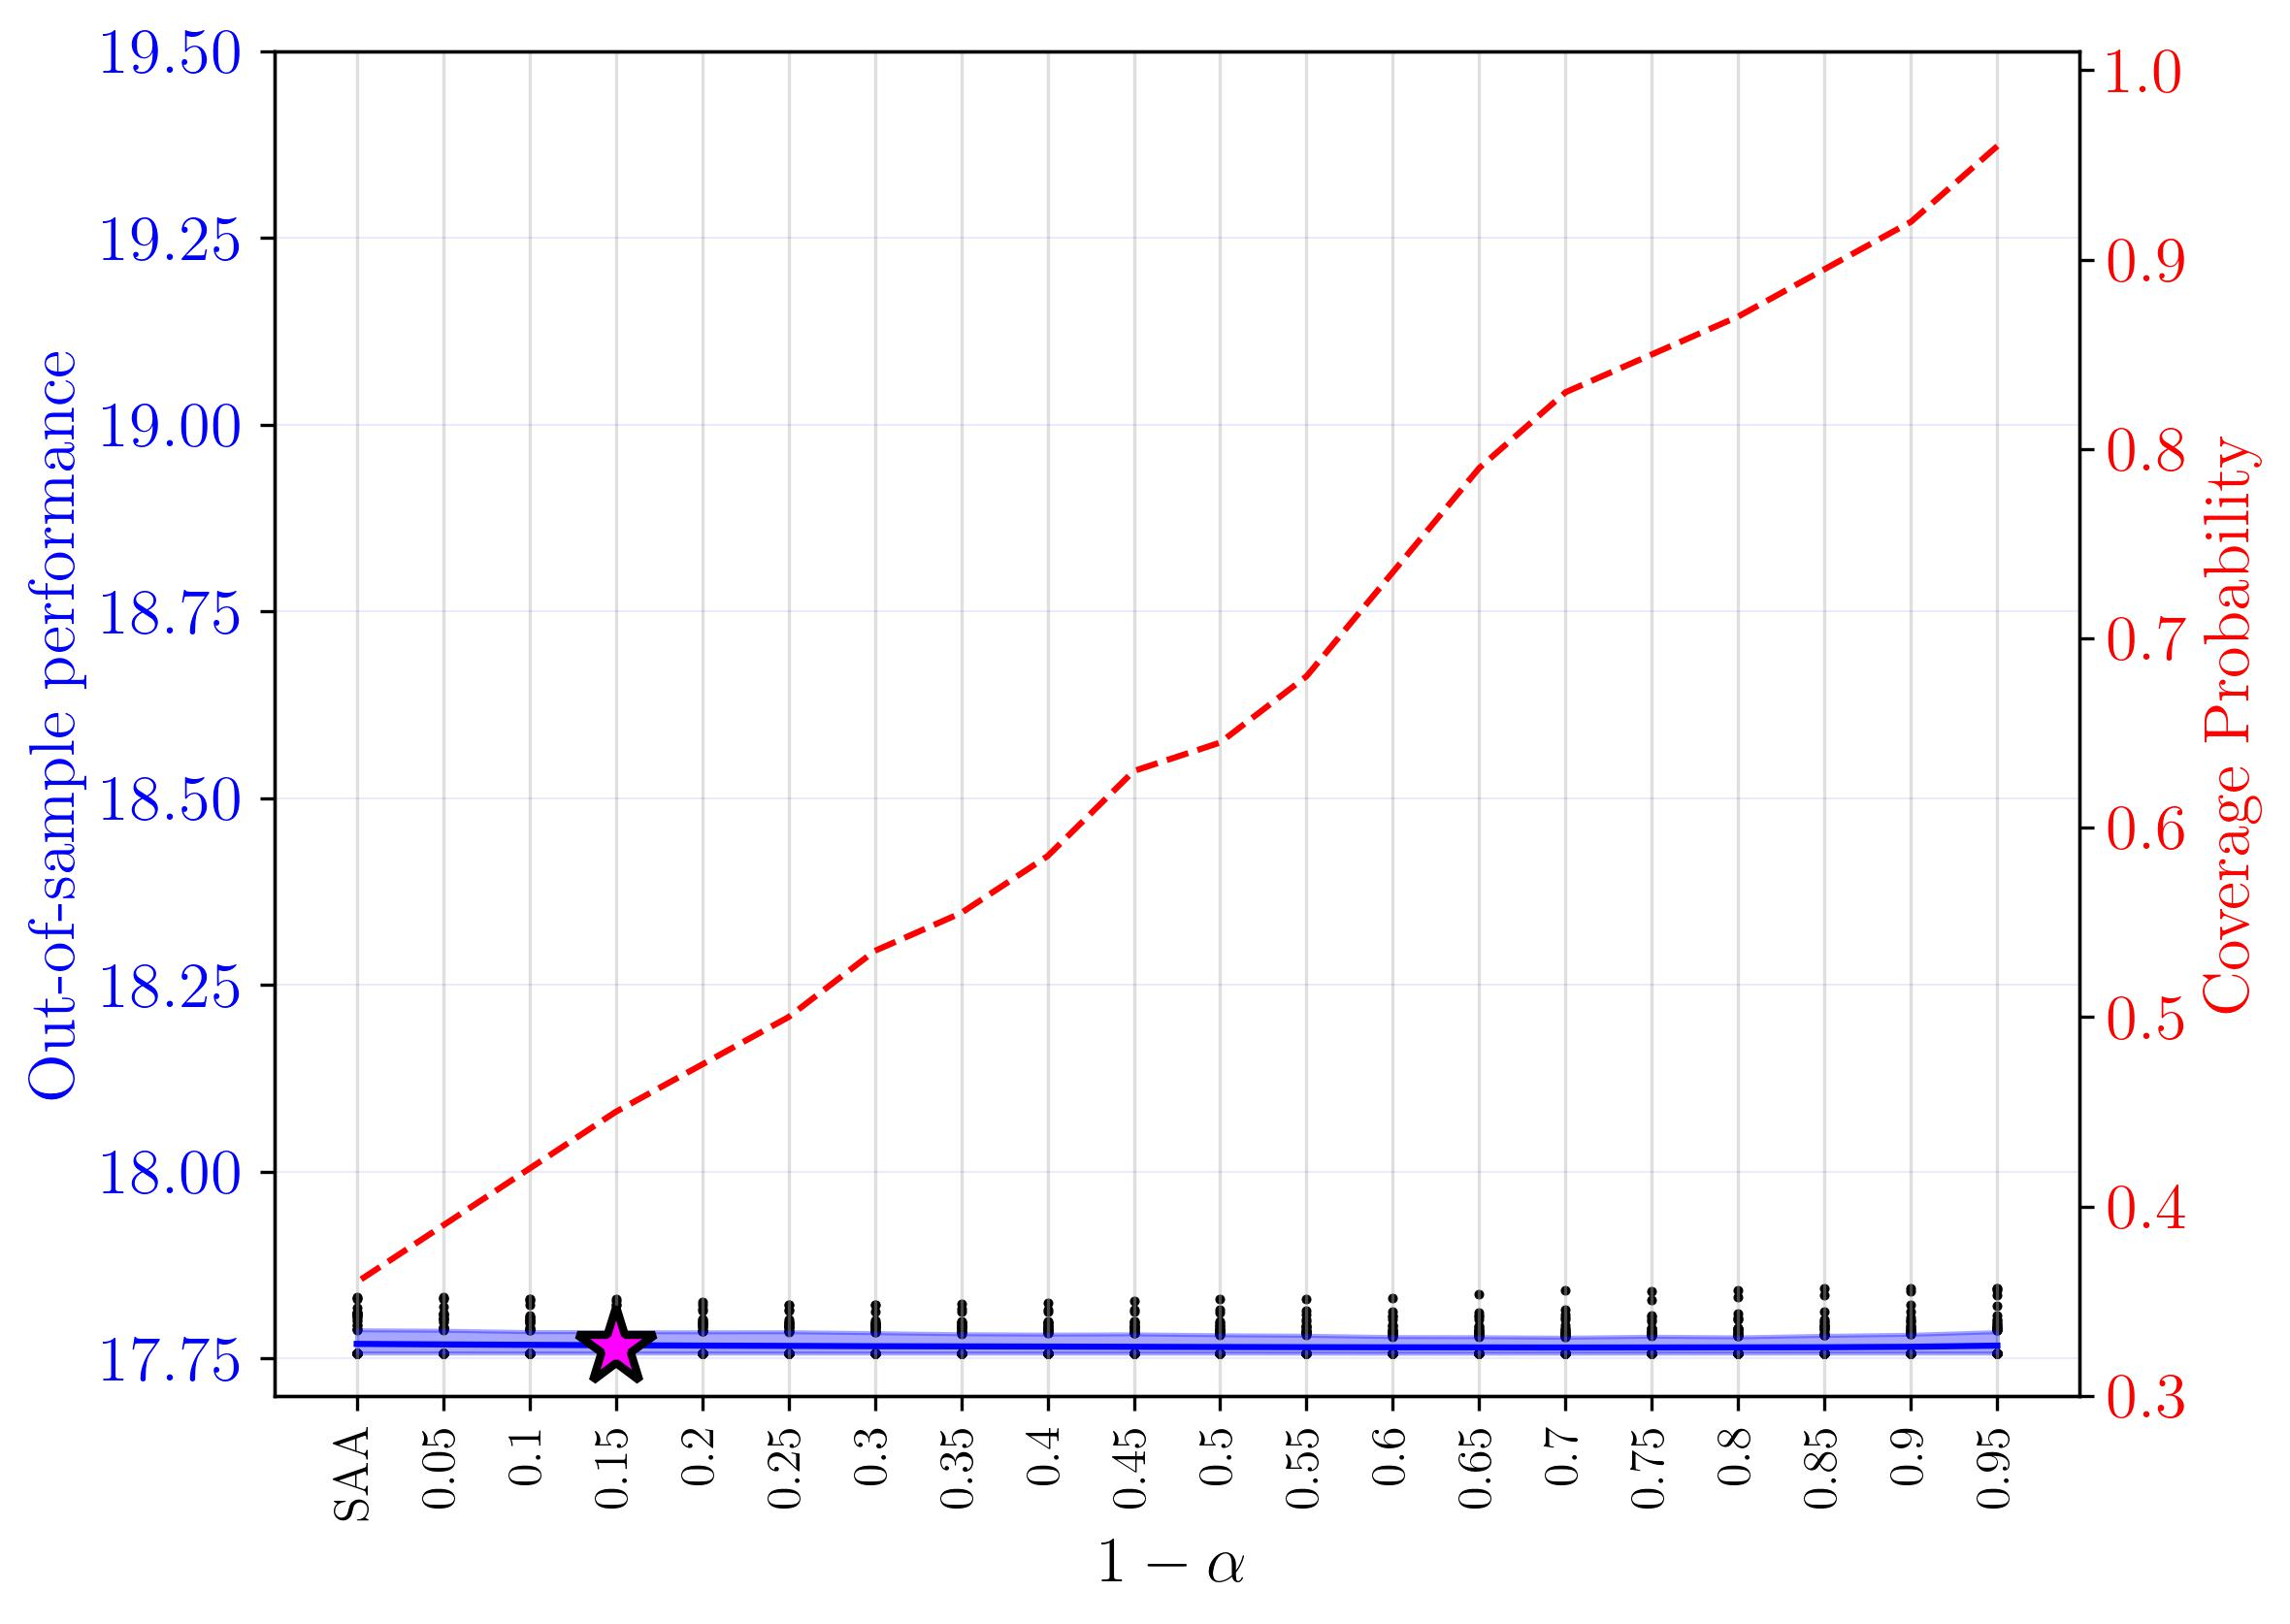
\includegraphics[width=0.33\textwidth]{performance_vs_reliability_alpha_640.jpg}
	}
		\caption{The optimal value of our model is \textbf{17.75}. We now compare the result for Out-of-sample performance (left axis, solid line, and shaded area) and the coverage probability (right axis, dashed line) as a function of the nominal confidence level $(1-\alpha)$ in APUB-SP. The star symbol indicates the point where the mean of the out-of-sample performance attains its minimum.  } \label{fig:RR-APUB} 
	\end{center}
\end{figure}



\newpage

%
%	\begin{equation}
%	\min_x \left\{ x + \mathbb{E}_p[Q(x, \xi)] : cx < B, \ x \geq 0 \right\},
%\end{equation}
%where the cost function $Q(x, \xi)$ is given by
%\begin{equation}
%	Q(x, \xi) := \min_y \left\{ s(D(\xi) - x - y)_+ + W(\xi)y : W(\xi)y + x \leq B, \ y \geq 0 \right\}.
%\end{equation}
%When $W(\xi)\le s$, $y = \frac{B-x}{W(\xi)}$
%\[
%Q(x,\xi)  = s\left(D(\xi) - x - \frac{B-x}{W(\xi)}\right)_+ + (B-x)
%\]
%When $W(\xi)> s$, $y = 0$
%\[
%Q(x,\xi)  = s(D(\xi)-x)
%\]
%Let $$p = \Pr(W(\xi)\le s).$$ Assuming independence, 
%\begin{align*}
%	\bE[Q(x,\xi)] &= p\bE\left[  s\left(D(\xi) - x - \frac{B-x}{W(\xi)}\right)_+ + (B-x)   \right] + (1-p)\bE[s(D(\xi)-x)] \\
%	&= sp \bE \left[  \left(D(\xi) - x - \frac{B-x}{W(\xi)}\right)_+   \right] + p(B-x) + s(1-p)(\mu_D - x) \\
%	& = sp \bE \left[  \left(D(\xi) - x - \frac{B-x}{W(\xi)}\right)_+   \right] + (pB+s(1-p)\mu_D) - (p+s(1-p))x
%\end{align*}
%Let $$q(x) = \Pr\left( D(\xi) - x - \frac{B-x}{W(\xi)}  \ge 0  \right)$$.
%Then,
%\[
%\bE \left[  \left(D(\xi) - x - \frac{B-x}{W(\xi)}\right)_+   \right]  = q(x) \left[ \mu_D -x  - \nu_{W} (B-x)  \right] = q(x) [(\nu_W-1)x + \mu_D - \nu_WB] .
%\]
%Thus,
%Let $F(x)$ be the objective function.
%\[
%F^\prime(x) = q^\prime(x)[(\nu_W-1)x + \mu_D - \nu_WB] + q(x)(\nu_W-1) - (p+s(1-p))+1
%\]

















\end{document}